\chapter{Задание}

В информационный центр приходят клиенты через интервалы времени $10\pm2$
минуты. Если все три имеющихся оператора заняты, клиенту отказывают в
обслуживании. Операторы имеют разную производительность и могут
обеспечивать обслуживание среднего запроса пользователя за $20\pm5$, $40\pm10$,
$40\pm20$ минут. Клиенты стремятся занять свободного оператора с максимальной
производительностью. 

Полученные запросы сдаются в приемный накопитель,
откуда они выбираются для обработки. На первый компьютер -- запросы от
первого и второго оператора, на второй компьютер -- от третьего оператора.
Время обработки на первом и втором компьютере равны соответственно 15 и 30
минутам.

Смоделировать процесс обработки 300 запросов. В результате определить вероятность отказа.
Необходимо построить структурную схему модели.

Нарисовать модель в терминах СМО.

\chapter{Математическая формализация}

\section{Структурная схема модели}

\noindent На рисунке \ref{fig:struct} представлена структурная схема модели.
\begin{figure}[H]
	\centering
	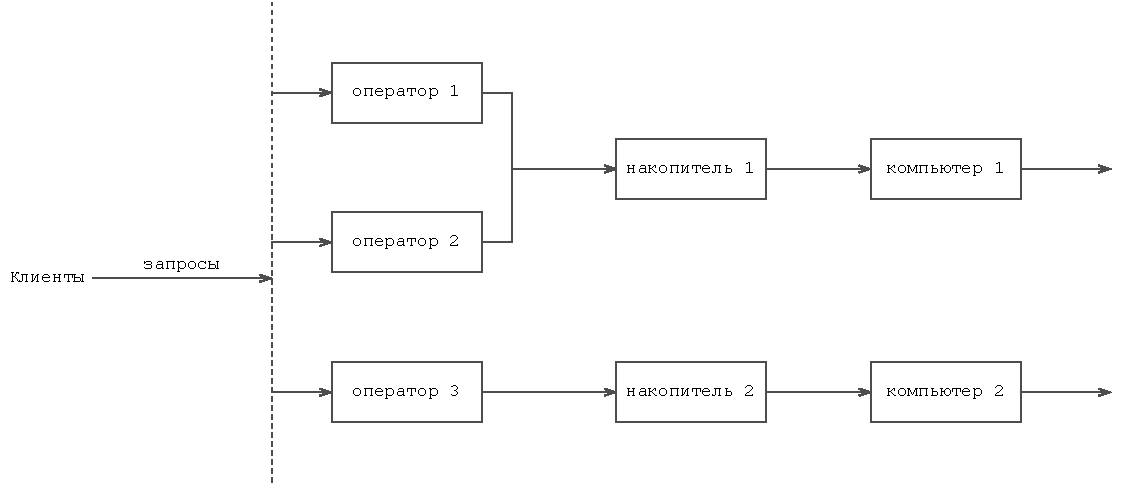
\includegraphics[width=0.8\textwidth]{assets/struct.pdf}
	\caption{Структурная схема модели}
	\label{fig:struct}
\end{figure}

\section{Концептуальная модель в терминах СМО}

\noindent На рисунке \ref{fig:smo} представлена концептуальная модель в терминах СМО.
\begin{figure}[H]
	\centering
	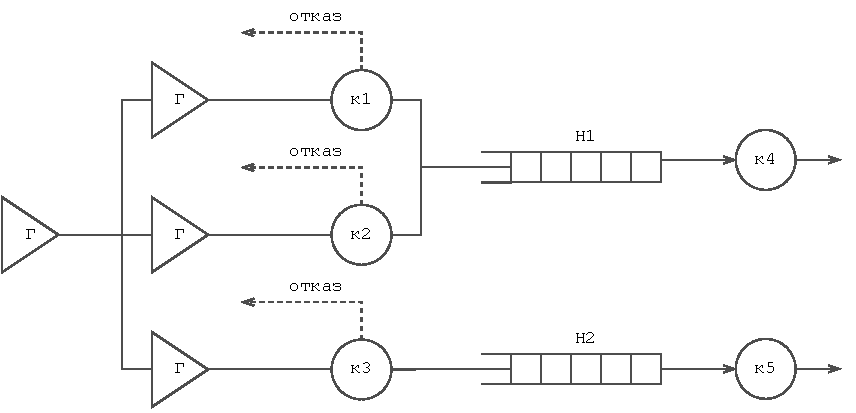
\includegraphics[width=0.8\textwidth]{assets/smo.pdf}
	\caption{Концептуальная модель в терминах СМО}
	\label{fig:smo}
\end{figure}

\noindent В процессе взаимодействия клиентов с информационным центром возможен:

\begin{itemize} 
	\item режим нормального обслуживания, т.е. клиент выбирает одного из свободных операторов, отдавая предпочтение тому у которого меньше номер.
	\item режим отказа в обслуживании клиента, когда все операторы заняты. 
\end{itemize}

\section{Переменные и уравнения модели}
\begin{itemize} 
	\item эндогенные переменные: время обработки задания i-ым оператором, время решения этого задания j-ым компьютером.
	\item экзогенные переменные: число обслуженных клиентов и число клиентов, получивших отказ.
\end{itemize}

Вероятность отказа в обслуживании выражается согласно \ref{rej}:

\begin{equation}\label{rej}
	P_{\text{отк}} = \frac{C_{\text{отк}}}{C_{\text{отк}} + C_{\text{обсл}}},
\end{equation}

где $C_\text{отк}$ -- число клиентов, получивших отказ, а $C_\text{обсл}$ -- число обслуженных клиентов.

